\chapter{불변 법칙, 4-벡터, 그리고 장 텐서}

먼저 자연이 따를 수도 있었지만 실제로는 따르지 않는 법칙을 살펴보자. 이 법칙이 성립하지 않는다는 사실은 물리 법칙을 어떻게 써야 하는지 알려준다. 같은 기준을 적용하면 먼저 좌표 성분에서 보통 벡터로, 이어서 보통 벡터에서 4-벡터로, 마지막으로 4-벡터에서 텐서로 나아가게 된다. 이 과정을 마치면 전기장과 자기장은 더 이상 서로 분리된 대상이 아니다. 두 장은 하나의 반대칭 텐서에서 서로 독립적인 여섯 성분을 이룬다.

달리 명시하지 않는 한 \(c=1\)인 단위를 사용하고, 시공간 성분의 순서를 \((1,2,3,0)=(x,y,z,t)\)로 하며, 계량 부호 규약은 \((-,-,-,+)\)로 둔다.

\section{대칭성이 잘못된 법칙의 한 예}

공간에 \(x\)축과 \(y\)축을 고정해 두자. 이제 두 입자의 \(x\)좌표가 일치할 때마다 입자들이 상호작용한다고 정해 보자. 이 상호작용으로 입자들의 운동 방향이 반대로 바뀌거나 새로운 방향으로 흩어질 수 있다. 구체적인 동역학은 중요하지 않다. 제안된 상호작용의 조건은 그저 \begin{equation}
  x_1-x_2=0,
\end{equation}이며, 아래 첨자는 좌표 성분이 아니라 입자를 가리킨다. 이 규칙에는 수학적 모순이 없다. 문제는 무엇 때문에 이 규칙을 물리적으로 타당하지 않다고 보는가이다.

\begin{classroomqa}\audiencequestion{이 규칙은 공간의 균질성을 위반하나요?}\lecturerresponse{아닙니다. 원점을 평행이동하면 두 좌표가 똑같은 양만큼 변하므로 \(x_1-x_2\)는 변하지 않습니다. 이 규칙은 특정 위치를 특별하게 취급하지 않습니다. 결함은 등방성에 있습니다. 특정 방향 하나를 특별하게 선택하기 때문입니다.}\end{classroomqa}

축을 \(90^\circ\)만큼 회전해 보자. 원래 \(x\)방향이라고 부르던 방향은 이제 \(y\)방향이므로, 같은 물리적 사건은 \(y\)좌표가 같다는 조건으로 기술된다. 일반적인 각도에서는 조건에 \(x\)와 \(y\)의 선형 결합이 들어간다. 따라서 법칙의 형태가 칠판을 어떤 방향으로 놓았는지에 따라 달라진다. 이 법칙은 평행이동에는 불변이지만 회전에는 불변이 아니다.

물리 법칙은 보통 직교 좌표계에서 가장 간단한 형태로 쓴다. 더 일반적인 좌표계를 쓸 수도 있지만, 그러면 계량과 식이 덜 간단해진다. 직교 데카르트 좌표계라는 범위 안에서는 어느 방향도 특별하게 취급해서는 안 된다.

수정 방법은 간단하다. 2차원에서는 두 좌표가 모두 일치하도록 하고, 3차원에서는 세 좌표가 모두 일치하도록 한다. \begin{equation}
  x_1=x_2,
  \qquad y_1=y_2,
  \qquad z_1=z_2.
\end{equation} 그러면 입자들은 서로 다른 직선을 따라 접근하더라도 같은 점에 도달할 때에만 상호작용할 수 있다.

\begin{classroomqa}\audiencequestion{\(z\)좌표와 시간도 일치해야 하나요?}\lecturerresponse{3차원 공간에서는 \(z\)좌표도 일치해야 합니다. 지금은 시간을 잠시 생략하지만, 공간에 관한 논의를 마치면 곧 다시 포함하겠습니다.}\end{classroomqa}

\(\boldsymbol r_a\)는 입자 \(a\)의 위치이다. 세 성분에 대한 조건은 하나의 벡터 방정식으로 나타낼 수 있다.
\begin{equation}
  \boldsymbol r_1-\boldsymbol r_2=\boldsymbol 0.
\end{equation}
어떤 회전 좌표계에서는 한 성분이 사라지지만, 다른 회전 좌표계에서는 사라지지 않을 수 있다. 벡터 전체에 대해서는 다르다. 한 좌표계에서 모든 성분이 사라지면 회전한 모든 좌표계에서도 모든 성분이 사라진다. 마찬가지로 한 좌표계에서 두 벡터가 같으면 둘 다 변환한 뒤에도 서로 같다.

\begin{figure}[H]\centering
\includegraphics[width=0.78\textwidth]{lecture_06_figure_01.png}\caption{충돌이 특정한 한 축을 따라 일치하는 것이 아니라 공간상의 일치를 뜻하게 하는 세 좌표의 등식.}\lectureframe{00:09:00}\end{figure}

벡터 방정식이 유용한 이유가 여기에 있다. 성분은 변하지만 대상 전체는 일관되게 변환된다. 전체 대상에 대해 쓴 법칙은 좌표계를 회전해도 형태를 유지할 수 있다.

\section{시공간에서의 일치}

이제 수직인 공간축을 시간으로 바꾸어 보자. 뉴턴 역학의 규칙은 두 운동 변화가 같은 시간에만 일어난다고 할 수 있다. 뉴턴 역학에서는 모든 관성 관찰자가 동시성을 공유하므로 그런 규칙이 가능하다. 특수 상대성 이론에서는 이 규칙이 특정 기준계를 선택한다. 한 기준계에서 동시인 사건들이 다른 기준계에서는 동시가 아닐 수 있다.

공간 좌표만 같다고 요구해도 나을 것이 없다. 시공간 변위는 공간 성분은 사라지고 시간 성분은 남는다.
\begin{equation}
  \Delta X^\mu=(0,0,0,\Delta t),
\end{equation}
부스트는 \(\Delta t\)와 공간 성분을 서로 섞는다. 불변인 국소적 진술은 두 운동 변화가 같은 사건에서 일어난다는 것이다. 따라서 단순한 충돌이 일어나려면 다음 조건이 필요하다.
\begin{equation}
  X_1^\mu=X_2^\mu,
  \qquad\text{or}\qquad
  X_1^\mu-X_2^\mu=0.
\end{equation}
네 좌표가 모두 일치한다. 즉 입자들은 같은 시각에 같은 위치를 차지한다.

충돌의 예는 물리학을 기술하는 일반적인 원칙을 보여준다. 모든 항을 한쪽에 모아 완전한 4-벡터를 0과 같게 두거나, 완전한 4-벡터 하나를 다른 하나와 같게 둘 수 있다. 4-벡터의 서로 연결되지 않은 일부만 같게 두는 것만으로는 로런츠 불변인 진술이 되지 않는다.

\section{부스트, 회전, 행렬 표기}

4-벡터란 시공간 변위와 같은 방식으로 변환되는 대상이다. 이 정의를 유용하게 쓰려면 먼저 좌표 자체의 변환을 떠올려야 한다. \(x\)방향으로 속력 \(v\)인 부스트의 경우, \begin{align}
  x'&=\gamma(x-vt), & y'&=y, & z'&=z,
  & t'&=\gamma(t-vx),                                      \label{eq:l6-boost}
\end{align} 여기서 \begin{equation}
  \gamma(v)=\frac{1}{\sqrt{1-v^2}}.
\end{equation}

\begin{classroomqa}\audiencequestion{이 식들에서는 빛의 속도를 1로 둔 건가요?}\lecturerresponse{그렇습니다. 단위를 복원하려면 \(X^0=ct\)로 놓고, \(1-v^2\)를 \(1-v^2/c^2\)로 바꾸며, 공간--시간 혼합항에 해당하는 \(c\)의 인자도 복원하면 됩니다.}\end{classroomqa}

\(z\)축 주위의 회전은 \(x\)와 \(y\)를 서로 섞고, \(z\)와 \(t\)는 그대로 둔다. \begin{equation}
\begin{pmatrix}
  x'\\ y'\\ z'\\ t'
\end{pmatrix}
=
\begin{pmatrix}
  \cos\theta & \sin\theta & 0 & 0\\
  -\sin\theta & \cos\theta & 0 & 0\\
  0 & 0 & 1 & 0\\
  0 & 0 & 0 & 1
\end{pmatrix}
\begin{pmatrix}
  x\\ y\\ z\\ t
\end{pmatrix}.
\end{equation} 영점도 표시할 필요가 있다. 변환된 좌표에 어떤 성분이 들어가지 않는지 분명하게 보여주기 때문이다. 같은 성분 순서로 쓰면 식~\eqref{eq:l6-boost}의 부스트는 다음과 같다. \begin{equation}
\begin{pmatrix}
  x'\\ y'\\ z'\\ t'
\end{pmatrix}
=
\begin{pmatrix}
  \gamma & 0 & 0 & -\gamma v\\
  0 & 1 & 0 & 0\\
  0 & 0 & 1 & 0\\
  -\gamma v & 0 & 0 & \gamma
\end{pmatrix}
\begin{pmatrix}
  x\\ y\\ z\\ t
\end{pmatrix}.
\end{equation}

회전과 부스트는 행렬 곱셈으로 합성할 수 있다. 원래 \(x\)축과 나란하지 않은 방향으로 부스트하려면, 그 방향이 \(x\)축과 나란해지도록 회전한 뒤 부스트를 적용하고 필요에 따라 다시 회전하면 된다. 이런 기본 행렬들의 곱으로 더 일반적인 로런츠 변환을 만들 수 있다.

\begin{classroomqa}\audiencequestion{먼저 회전한 뒤 부스트하는 것과 먼저 부스트한 뒤 회전하는 것은 차이가 있나요?}\lecturerresponse{있습니다. 첫 번째 연산을 거치면 두 번째 연산이 작용하는 축이 바뀝니다. 따라서 두 행렬 곱은 같지 않을 수 있고, 연산 순서가 중요합니다.}\end{classroomqa}

이 모든 선형 변환을 한꺼번에 다음과 같이 쓸 수 있다. \begin{equation}
  X'^{\mu}=\Lambda^{\mu}{}_{\nu}X^{\nu}.                  \label{eq:l6-vector-transform}
\end{equation} 반복되는 첨자 \(\nu\)에 대해서는 \(1,2,3,0\)에 걸쳐 합한다. 이는 행렬 곱셈에서 행과 열의 원소를 곱해 더하는 통상적인 계산을 첨자 표기로 나타낸 것이다.

\begin{figure}[H]\centering
\includegraphics[width=0.78\textwidth]{lecture_06_figure_02.png}\caption{열벡터 형태로 쓰기 전의 로런츠 변환 첨자 표기.}\lectureframe{00:31:55}\end{figure}

식~\eqref{eq:l6-vector-transform}은 일반적인 반변 4-벡터의 정의이기도 하다. \(A^\mu\)가 그런 벡터라면 다음과 같이 변환된다. \begin{equation}
  A'^{\mu}=\Lambda^{\mu}{}_{\nu}A^{\nu}.
\end{equation} 네 성분이 위치를 나타낼 필요는 없다. 이 대상이 4-벡터인 까닭은 그 변환 법칙에 있다.

\section{스칼라, 계량, 불변 곱}

4-벡터를 더 다루기 전에 한 걸음 물러나 스칼라라는 더 간단한 개념을 살펴보면 도움이 된다. 공간상의 특정 지점에서의 온도는 스칼라이며, 두 특정 지점 사이의 거리도 스칼라이다. 각각은 축의 방향과 무관한 하나의 수이다. 일부러 우스꽝스럽게, 센티미터로 잰 거리가 화씨 온도로 잰 실내 온도와 같다고 주장할 수도 있다. 물리적으로 의미 있는 주장은 아니지만, 양변이 모두 회전 스칼라이므로 축을 어떻게 돌리든 그 주장의 참과 거짓은 달라지지 않는다.

벡터의 성분은 스칼라가 아니다. 따라서 성분을 스칼라로 결합하는 체계적인 방법이 필요하다. 일반적인 반변 4-벡터를 다음과 같이 쓰자. \begin{equation}
  A^\mu=(A^1,A^2,A^3,A^0).
\end{equation} 공변 성분은 같은 기하학적 대상을 아래 첨자로 나타낸 것이다. 우리가 쓰는 부호 규약에서는 민코프스키 계량을 사용해 다음과 같이 구한다. \begin{equation}
  A_\mu=\eta_{\mu\nu}A^\nu,
  \qquad
  \eta_{\mu\nu}=
  \begin{pmatrix}
    -1&0&0&0\\
    0&-1&0&0\\
    0&0&-1&0\\
    0&0&0&1
  \end{pmatrix},                                          \label{eq:l6-metric}
\end{equation} 따라서 \begin{equation}
  A_\mu=(-A^1,-A^2,-A^3,A^0).
\end{equation}

\begin{classroomqa}\audiencequestion{칠판에 쓴 첨자와 부호 둘이 서로 맞지 않나요?}\lecturerresponse{맞습니다. 표시된 열벡터의 공간 성분에는 해당하는 음의 부호가 필요합니다. 첨자를 내리는 식에서 계량 \(\eta_{\mu\nu}\)을 곱하기 전 오른쪽 성분들의 첨자는 위쪽이어야 합니다. 시간 성분의 첨자는 \(0\)이지 \(4\)가 아닙니다.}\end{classroomqa}

\begin{figure}[H]\centering
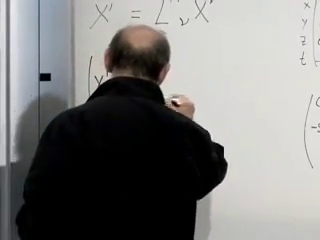
\includegraphics[width=0.8\textwidth]{lecture_06_figure_03.png}\caption{반변 성분과 공변 성분, 계량 행렬, 그리고 불변 수축의 시작.}\lectureframe{00:45:00}\end{figure}

첨자를 내리는 것은 단순한 표기상의 장식이 아니다. 로런츠 불변 노름에 필요한 부호를 반영한다. \begin{align}
  A_\mu A^\mu
  &=-(A^1)^2-(A^2)^2-(A^3)^2+(A^0)^2,                    \label{eq:l6-norm}\\
  X_\mu X^\mu
  &=t^2-x^2-y^2-z^2.
\end{align} 두 번째 식은 원점에서부터의 불변 시공간 간격이다. \(A^\mu\)가 \(X^\mu\)와 같은 방식으로 변환하므로 그 수축은 불변이다.

이 표기는 유용한 계산 규칙도 알려준다. 합산되는 첨자는 위에 한 번, 아래에 한 번 나타난다. 예를 들면 다음과 같다. \begin{equation}
  A_\mu A^\mu
  =\eta_{\mu\nu}A^\mu A^\nu.
\end{equation} 합산 첨자, 즉 더미 첨자의 이름은 양을 바꾸지 않고 바꿀 수 있다.

\begin{classroomqa}\audiencequestion{이 벡터 중 하나를 행으로, 다른 하나를 열로 봐야 하나요? 그리고 순서가 중요한가요?}\lecturerresponse{현재 계산에서는 첨자가 붙은 양을 성분으로 보고 계량으로 수축하면 됩니다. 논의를 행과 열의 연산자 대수로 바꿀 필요는 없습니다. 이들은 보통 수이므로 순서는 중요하지 않습니다. 교환하지 않는 연산자라면 더 주의해야 하지만, 여기서는 그런 내용을 다루지 않습니다.}\end{classroomqa}

같은 구성으로 서로 다른 두 4-벡터 사이의 내적을 얻을 수 있다. \begin{equation}
  A\mathbin{\cdot}B=A_\mu B^\mu=A^\mu B_\mu.
\end{equation} 로런츠 행렬을 명시적으로 쓰지 않고도 이 내적이 불변임을 보일 수 있다. \(A+B\)와 \(A-B\)가 4-벡터이므로 두 제곱 노름은 모두 불변이다. \begin{align}
  (A+B)^2&=A^2+B^2+2A\mathbin{\cdot}B,\\
  (A-B)^2&=A^2+B^2-2A\mathbin{\cdot}B.
\end{align} 두 식을 빼면 다음을 얻는다. \begin{equation}
  (A+B)^2-(A-B)^2=4A\mathbin{\cdot}B,                    \label{eq:l6-polarization}
\end{equation} 따라서 \(A\mathbin{\cdot}B\)도 불변이다. 인수 4는 전개에서 바로 나온다.\editorialnote{칠판의 논증은 이 편극 항등식을 보여준다. 인수를 직접 적어 두면 말로 설명한 소거 과정이 모호하지 않다.}

\begin{figure}[H]\centering
\includegraphics[width=0.8\textwidth]{lecture_06_figure_04.png}\caption{서로 다른 4-벡터의 내적을 분리해 구하는 데 쓰인 두 불변 제곱식.}\lectureframe{00:52:20}\end{figure}

불변량은 물리 법칙에 자연스럽게 들어간다. 고립된 성분과 달리 기준계가 바뀌어도 같은 값을 유지하기 때문이다.

\section{고유 속도와 4-운동량}

입자의 세계선 위에서 서로 이웃한 두 사건을 생각하자. 두 사건의 간격은 미소 4-벡터이다. \begin{equation}
  dX^\mu=(dx,dy,dz,dt).
\end{equation} 시간꼴 세계선에 대해서는 고유시간을 다음과 같이 정의한다. \begin{equation}
  d\tau^2=dX_\mu dX^\mu
  =dt^2-dx^2-dy^2-dz^2.                                  \label{eq:l6-proper-time}
\end{equation} 고유 4-속도는 다음과 같다. \begin{equation}
  U^\mu=\frac{dX^\mu}{d\tau}.                            \label{eq:l6-four-velocity}
\end{equation} 이는 특정 기준계의 좌표 시간이 아니라 입자 자신의 고유시간에 대한 시공간 위치의 변화율이다.

\(U^\mu\)에는 성분이 네 개 있지만 독립적인 성분은 세 개뿐이다. 식~\eqref{eq:l6-proper-time}을 \(d\tau^2\)으로 나누면 다음을 얻는다. \begin{equation}
  U_\mu U^\mu=1.
\end{equation} 따라서 4-속도는 단위 시간꼴 벡터이다. 미래 방향을 택하면 시간 성분의 부호가 정해진다.

\begin{classroomqa}\audiencequestion{\(c\)보다 훨씬 느린 속도에서는 4-속도가 보통 속도로 줄어드나요?}\lecturerresponse{공간 성분 세 개는 보통 속도에 가까워지고, 시간 성분은 \(c=1\) 단위에서 1에 가까워집니다. 연쇄 법칙을 적용하고 \(dt/d\tau\)을 계산하면 이 관계를 얻습니다.}\end{classroomqa}

각 공간 성분에 대해 다음이 성립한다. \begin{equation}
  U^i=\frac{dx^i}{d\tau}
     =\frac{dx^i}{dt}\frac{dt}{d\tau}
     =v^i\frac{dt}{d\tau}.
\end{equation} 식~\eqref{eq:l6-proper-time}을 \(dt^2\)으로 나누면 다음과 같다. \begin{equation}
  \left(\frac{d\tau}{dt}\right)^2
  =1-v_x^2-v_y^2-v_z^2
  =1-\boldsymbol v^2.
\end{equation} 따라서 \begin{equation}
  \frac{dt}{d\tau}=\frac{1}{\sqrt{1-\boldsymbol v^2}}
  =\gamma(\lvert\boldsymbol v\rvert),
\end{equation}이고, \begin{equation}
  U^\mu=(\gamma v_x,\gamma v_y,\gamma v_z,\gamma).
                                                                  \label{eq:l6-u-components}
\end{equation}

\begin{figure}[H]\centering
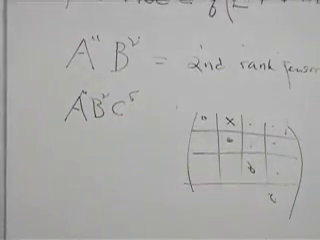
\includegraphics[width=0.8\textwidth]{lecture_06_figure_05.png}\caption{고유시간 계산으로 \(dt/d\tau=\gamma\)을 구하고 고유 속도와 보통 속도의 관계를 나타낸다.}\lectureframe{01:02:00}\end{figure}

\begin{classroomqa}\audiencequestion{\(dx^2/dt^2\)는 이계도함수를 뜻하나요? 벡터를 제곱하면 교차항이 생겨야 하지 않나요?}\lecturerresponse{여기서는 일계도함수의 제곱인 \((dx/dt)^2\)를 뜻합니다. 또 \(\boldsymbol v^2\)은 유클리드 내적 \(v_x^2+v_y^2+v_z^2\)을 뜻하지 형식적인 합 \(v_x+v_y+v_z\)의 제곱을 뜻하지 않으므로 교차항은 없습니다.}\end{classroomqa}

\begin{classroomqa}\audiencequestion{\(v\)는 \(\gamma(v)\)에서 두 기준계 사이의 상대 속도인가요, 아니면 입자의 속도인가요?}\lecturerresponse{여기서는 선택한 기준계에서 본 입자의 속도입니다. 함수 \(\gamma(v)=1/\sqrt{1-v^2}\)는 어떤 속도에 대해서도 계산할 수 있습니다. 부스트에서는 기준계 사이의 상대 속도를 대입하고, 4-속도에서는 입자의 속도를 대입합니다.}\end{classroomqa}

\(v\ll1\)이면 \(\gamma\simeq1\)이므로 \(U^\mu\)의 공간 성분은 \(\boldsymbol v\)에 가까워지고 \(U^0\)은 1에 가까워진다. 보통 속도가 빛의 속도에 가까워지면 \(\gamma\)는 커지고 사차원 속도의 0이 아닌 모든 성분은 한없이 커진다.

\begin{classroomqa}\audiencequestion{\(U^0\)는 1에 가까운 수가 아니라 속도의 단위를 가져야 하지 않나요?}\lecturerresponse{\(c\)를 1로 두면서 단위가 사라졌습니다. \(X^0=ct\)를 사용하면 \(U^\mu=(\gamma\boldsymbol v,\gamma c)\)이므로 시간 성분은 \(c\)에 가까워지고 \(U_\mu U^\mu=c^2\)가 됩니다.}\end{classroomqa}

정지 질량이 \(m\)인 입자의 4-운동량을 다음과 같이 정의하자. \begin{equation}
  P^\mu=mU^\mu.
\end{equation} 자연 단위계에서는 \begin{equation}
  P^\mu=(\gamma m\boldsymbol v,\gamma m).
\end{equation} 저속에서 처음 세 성분은 뉴턴 역학의 운동량 \(m\boldsymbol v\)에 가까워진다. 단위를 복원하면 다음과 같다. \begin{equation}
  P^\mu=(\gamma m\boldsymbol v,E/c),
  \qquad E=\gamma mc^2,
\end{equation} 따라서 \begin{equation}
  E=mc^2+\frac{1}{2}m\boldsymbol v^2+O(mv^4/c^2).
\end{equation} 시간 성분은 \(c=1\) 단위계에서 에너지이며, 네 성분 모두에 운동량 단위를 부여하면 에너지를 \(c\)로 나눈 값이다.

\begin{classroomqa}\audiencequestion{\(\boldsymbol v\)의 끝에 네 번째 성분을 붙인 것 자체가 4-벡터인가요?}\lecturerresponse{아닙니다. 보통 3-속도는 4-벡터처럼 변환되지 않습니다. 인자 \(\gamma\)와 고유시간을 이용한 정의가 필수입니다. 4-벡터는 \(U^\mu\)이지 \(\boldsymbol v\)가 아닙니다.}\end{classroomqa}

\section{전기장과 자기장이 서로 섞여야 하는 이유}

이제 상대성 이론을 잠시 쉬어 간다. 아인슈타인 이전의 운동 방정식에서 시작해, 모든 관성 기준계에서 성립하려면 이 방정식을 어떻게 다시 구성해야 하는지 살펴보자. 보통 가속도는 보통 속도의 시간 미분이다. 이에 대응하는 4차원 양은 자연스럽게 다음과 같다. \begin{equation}
  A^\mu=\frac{dU^\mu}{d\tau}.
\end{equation} 저속에서는 그 공간 성분이 보통 가속도에 가까워진다. 완전한 상대론적 방정식은 뒤로 미루고, 먼저 옛 힘 법칙을 살펴보자.

전기장과 자기장 속의 전하 \(q\)에 대해 \begin{equation}
  \boldsymbol F=m\boldsymbol a
  =q\left(\boldsymbol E+\boldsymbol v\times\boldsymbol B\right).
                                                                  \label{eq:l6-lorentz-force}
\end{equation} 전기력 항은 입자 속도와 무관하지만 자기력 항은 그렇지 않다.

\begin{figure}[H]\centering
\includegraphics[width=0.8\textwidth]{lecture_06_figure_06.png}\caption{\(\boldsymbol E\)과 \(\boldsymbol B\)를 결합해야 하는 이유가 되는 상대론 이전의 로런츠 힘 법칙.}\lectureframe{01:18:20}\end{figure}

관측자가 전기장은 없고 자기장과 움직이는 전하는 있다고 본다고 하자. 전하는 자기력을 받는다. 그러나 전하의 순간 정지 좌표계에서는 \(\boldsymbol v=0\)이므로 식~\eqref{eq:l6-lorentz-force}의 자기 항은 사라진다. 좌표계가 바뀌었다고 해서 물리적 세계선이 관성 운동을 하게 된 것은 아니다. 따라서 새 좌표계에서 힘에는 전기력에 해당하는 항이 포함되어야 한다. 더 정확히 말하면, 관성 좌표계 사이의 변환으로 4-가속도를 0으로 만들 수는 없다. 다만 보통의 3-가속도와 그 성분은 변환된다.
\editorialnote{4-가속도에 관한 이 진술은 강의실 논증을 불변인 형태로 나타내며, 보통의 3-가속도 자체를 좌표계에 무관한 양으로 취급하지 않도록 해 준다.}

따라서 전기장과 자기장은 서로 변환되어야 한다. 두 장을 합치면 성분이 여섯 개이므로 하나의 스칼라도, 하나의 4-벡터도 아니다. 새로운 변환 대상을 도입해야 한다.

\section{텐서: 첨자마다 하나씩 변환}

스칼라는 계수가 0인 텐서라고 부를 수 있으며 첨자가 없다. 4-벡터는 계수가 1인 텐서이며, 네 가지 값을 가질 수 있는 첨자 하나를 갖는다. 가장 간단한 계수 2의 예는 다음과 같은 곱이다. \begin{equation}
  A^\mu B^\nu.
\end{equation} 각 첨자는 네 가지 값을 가지므로 이 대상은 \(4^2=16\)개의 성분을 가지며, \(4\times4\) 배열로 나타낼 수 있다. 세 벡터의 곱 \begin{equation}
  A^\mu B^\nu C^\sigma,
\end{equation}은 \(4^3=64\)개의 성분을 가지는 계수 3 텐서이다. 더 높은 계수에서도 이 패턴이 이어진다. 이름보다 중요한 것은 대상을 정의하는 규칙이다.

다음과 같다고 하자. \begin{equation}
  A'^{\mu}=\Lambda^\mu{}_{\nu}A^\nu,
  \qquad
  B'^{\sigma}=\Lambda^\sigma{}_{\tau}B^\tau,
\end{equation} 그러면 그 곱은 다음과 같이 변환된다. \begin{equation}
  A'^{\mu}B'^{\sigma}
  =\Lambda^\mu{}_{\nu}\Lambda^\sigma{}_{\tau}
   A^\nu B^\tau.
\end{equation} 이로부터 반변 계수 2 텐서의 정의 법칙을 얻는다. \begin{equation}
  T'^{\mu\sigma}
  =\Lambda^\mu{}_{\nu}\Lambda^\sigma{}_{\tau}T^{\nu\tau}.
                                                                  \label{eq:l6-tensor-transform}
\end{equation} 각 첨자마다 로런츠 행렬 하나가 들어간다. 반복되는 \(\nu\)와 \(\tau\)에 대해서는 합산하고, 열린 첨자 \(\mu\)와 \(\sigma\)는 프라임 기준계에서 계산하는 성분을 나타낸다.

\begin{figure}[H]\centering
\includegraphics[width=0.82\textwidth]{lecture_06_figure_07.png}\caption{두 벡터의 변환과 그에 따른 계수 2 텐서의 두 행렬 변환 법칙.}\lectureframe{01:27:15}\end{figure}

텐서가 반드시 벡터들의 단일 곱일 필요는 없다. \(A^\mu B^\nu\)와 \(A^\nu B^\mu\)는 모두 텐서 변환 법칙을 따르며, 이들의 합이나 다음과 같은 합도 마찬가지다. \begin{equation}
  A^\mu B^\nu+C^\mu D^\nu.
\end{equation} 정의는 특정한 인수분해가 아니라 변환 법칙이다. 계수 3 텐서에는 로런츠 행렬이 하나 더 붙으며, 그 이상의 계수에서도 같은 방식으로 이어진다.

\section{대칭 텐서와 반대칭 텐서}

계수 2 텐서 가운데 두 종류가 특히 유용하다. 대칭 텐서는 다음을 만족한다. \begin{equation}
  T^{\mu\nu}=T^{\nu\mu},
\end{equation} 따라서 대각선을 사이에 두고 마주 보는 성분은 서로 같다. 대각 성분 네 개와 대각선 한쪽의 성분 여섯 개로 나머지를 정할 수 있으므로, 독립 성분은 \begin{equation}
  4+6=10
\end{equation}개이다.

반대칭 텐서는 다음 조건을 만족한다.
\begin{equation}
  T^{\mu\nu}=-T^{\nu\mu}.                                \label{eq:l6-antisymmetry}
\end{equation}
\(\mu=\nu\)를 식~\eqref{eq:l6-antisymmetry}에 대입하면 \(T^{\mu\mu}=-T^{\mu\mu}\)이므로 모든 대각 성분은 0이다. 삼각형 모양의 한쪽 절반에 있는 여섯 성분으로 부호만 바꾸어 반대쪽 나머지 여섯 성분을 정할 수 있다. 따라서 독립 성분은 정확히 여섯 개이다.

\begin{figure}[H]
\centering
\includegraphics[width=0.82\textwidth]{lecture_06_figure_08.png}
\caption{완성된 반대칭 \(4\times4\) 배열: 대각선 원소는 0이고, 대각선을 기준으로 서로 마주 보는 원소들의 부호는 반대이다.}
\lectureframe{01:34:25}
\end{figure}

이 개수가 단서다. 전기장의 세 성분과 자기장의 세 성분을 하나의 반대칭 계수 2 텐서에 담을 수 있다.

\section{전자기장 텐서}

시공간 첨자를 행과 열에 \((1,2,3,0)=(x,y,z,t)\)의 순서로 배치하자. 칠판에 쓴 배열은 다음과 같다. \begin{equation}
  F_{\mu\nu}=
  \begin{pmatrix}
    0    & -B_3 & B_2  & E_1\\
    B_3  & 0    & -B_1 & E_2\\
    -B_2 & B_1  & 0    & E_3\\
    -E_1 & -E_2 & -E_3 & 0
  \end{pmatrix}.                                         \label{eq:l6-field-tensor}
\end{equation} 순수한 공간 첨자가 붙은 성분에는 자기장이 들어가고, 공간 첨자 하나와 시간 첨자 하나가 붙은 성분에는 전기장이 들어간다. 반대칭성에 따라 위쪽 삼각형의 성분을 알면 아래쪽 삼각형의 성분도 정해진다.

\begin{classroomqa}\audiencequestion{자기장 성분은 모두 음수인가요? 첨자가 \(x,y,z\)에 대응하나요?}\lecturerresponse{위쪽 공간 삼각형에서 부호는 다음과 같이 번갈아 나타납니다. \(-B_3,+B_2,-B_1\) 첨자 \(1,2,3\)는 \(x,y,z\)에 대응하고, 첨자 \(0\)는 시간을 나타냅니다. 대각선을 사이에 두고 반사하면 모든 부호가 바뀝니다.}\end{classroomqa}

\begin{figure}[H]\centering
\includegraphics[width=0.82\textwidth]{lecture_06_figure_09.png}\caption{공간 성분을 먼저 쓰는 강의의 성분 순서로 완성한 전자기장 텐서.}\lectureframe{01:41:05}\end{figure}

표기법은 보통 일반적인 \(T_{\mu\nu}\)가 아니라 \(F_{\mu\nu}\)로 쓴다. 강연자는 이 문자가 패러데이를 가리킬 수도 있다고 추측하지만, 표기의 유래는 모른다고 분명히 말한다. 여기서 중요한 것은 문자의 유래에 관한 추측이 아니라 텐서의 반대칭성과 여섯 개의 장 성분이다.

\begin{classroomqa}\audiencequestion{각 행렬 성분은 표시된 좌표 평면에서의 장의 세기를 나타내나요?}\lecturerresponse{각 성분은 전자기장 텐서의 성분입니다. 시간 첨자가 들어가는 성분은 전기 성분이고, 공간--공간 성분은 자기 성분을 나타냅니다.}\end{classroomqa}

시간 첨자가 붙은 행과 열을 분리해 두면, 나머지 \(3\times3\) 반대칭 블록은 자기장에 해당한다. 독립 성분은 다음 순환 관계로 기억할 수 있다.
\begin{equation}
  F_{12}=-B_3,
  \qquad F_{23}=-B_1,
  \qquad F_{31}=-B_2.                                   \label{eq:l6-magnetic-cycle}
\end{equation}
첫 번째 관계에서 시작해 모든 첨자를 \(1\to2\to3\to1\) 순서로 차례로 바꾸면 된다. 이를 동등하게 다음과 같이 쓸 수 있다.
\begin{equation}
  F_{ij}=-\epsilon_{ijk}B_k,
\end{equation}
여기서 \(\epsilon_{123}=+1\)이다.\editorialnote{레비--치비타 공식은 칠판에서 명시적으로 전개한 순환 규칙을 간결하게 나타내는 표준형이다.}

\begin{figure}[H]\centering
\includegraphics[width=0.82\textwidth]{lecture_06_figure_10.png}\caption{반대칭 텐서에서 자기장을 나타내는 공간 성분들의 순환 관계.}\lectureframe{01:46:20}\end{figure}

전기장의 대응 관계는 더 직접적이다. \begin{equation}
  E_1=F_{10},
  \qquad E_2=F_{20},
  \qquad E_3=F_{30}.
\end{equation}

따라서 자기장은 두 가지 방식으로 표현할 수 있다. 3차원 공간에서는 성분 세 개를 가진 축벡터를 \(3\times3\) 반대칭 텐서와 짝지을 수 있다. 그러나 시공간에서는 자기장이 6성분 텐서 \(F_{\mu\nu}\)의 공간 부분에 불과하다. 성분이 \(4\times4\)개인 반대칭 텐서를 4-벡터와 동일시할 수 없으므로, 이 대응은 3차원에만 특별히 성립한다.\editorialnote{정회전에서는 자기장이 벡터처럼 변환되지만, 반사에서는 더 정확히 축벡터 또는 유사벡터로 변환된다.}

이 구성을 도입한 목적은 단순히 성분을 세는 데 있지 않다. \(F_{\mu\nu}\)가 텐서로 변환되므로 로런츠 부스트는 그 전기 성분과 자기 성분을 자동으로 서로 섞는다. 다음 강의에서는 이를 4-속도 및 4-가속도와 결합해 식~\eqref{eq:l6-lorentz-force}을 공변 운동 방정식으로 바꿀 수 있다.

\section{아인슈타인과 민코프스키에 관한 질문}

마지막 몇 분은 형식론에서 그 역사적 기원에 관한 이야기로 넘어간다. 여기서 제시하는 답은 확정된 역사라기보다 회고에 따른 것이며, 그 단서 역시 이 문답의 일부다.

\begin{classroomqa}\audiencequestion{아인슈타인은 개념적인 이유로 로런츠 불변 형식을 찾았나요, 아니면 특정 관측에 이끌렸나요?}\lecturerresponse{자연 법칙은 모든 관성 기준계에서 같은 형태를 가져야 한다는 원리가 그의 추론에서 핵심이었다. 에테르를 통한 운동을 검출하지 못한 사실과 빛에 관한 실험 증거도 있었지만, 강연자는 아인슈타인이 어떤 결과를 알고 있었는지, 또는 그 결과가 그에게 어느 정도 영향을 미쳤는지는 분명히 확신하지 못한다고 말한다. 개념적인 압력은 맥스웰 방정식과 로런츠 힘이 상대성 원리를 따라야 한다는 데 있었다. 그러려면 전기장, 자기장, 속도 성분이 함께 변환되어야 한다.}\end{classroomqa}

아인슈타인의 1905 논문에는 여기서 쓰는 간결한 4-벡터 표기가 없었다. 필요한 \(\gamma\) 인자와 속도를 명시적으로 적어 성분별로 전개했다. 이후 민코프스키는 같은 구조를 4차원 시공간의 기하학으로 정리했다.

\begin{classroomqa}\audiencequestion{아인슈타인은 민코프스키의 시공간 형식에 반대했나요? 민코프스키가 이를 도입한 시점은 언제인가요?}\lecturerresponse{강의에서 나온 회고에 따르면 아인슈타인은 처음에는 4차원 기하학 언어를 반기지 않았지만, 그 가치를 곧 받아들였다. 도입 시점은 1905 논문이 나온 뒤 대략 2년, 아마 1907 무렵이라고 잠정적으로 제시한다. 강연자는 역사를 확정하는 것이 아니라 회고하는 것이라고 강조한다.}\end{classroomqa}

\begin{classroomqa}\audiencequestion{민코프스키는 수학자였나요, 물리학자였나요? 또 어떤 업적을 남겼고, 로런츠나 피츠제럴드의 영향을 받았나요?}\lecturerresponse{확실한 답을 내놓지는 않는다. 수학자와 물리학자를 구분하는 문제는 더 다루지 않았고, 청중의 정정이 민코프스키의 다른 업적에 대한 포괄적인 언급을 끊는다. 가능한 영향 관계에 대해서도 명시적으로 확신하지 못한다고 한다. 이 논의에서 확실한 점은 민코프스키가 상대성 이론을 4차원 기하학 표기로 정리하는 데 결정적인 역할을 했다는 것이다.}\end{classroomqa}

\begin{classroomqa}\audiencequestion{\(\boldsymbol E\)와 \(\boldsymbol B\)를 서로 섞는 변환은 아인슈타인의 1905 논문에 이미 있었나요?}\lecturerresponse{있었습니다. 다만 하나의 장 텐서 방정식으로 쓰지 않고 성분별로 적었습니다. 강의에서는 이를 맥스웰 방정식의 성분별 표현과 비교한다. 공통 구조를 드러내는 간결한 표기법이 나오기 전에도 그 내용은 담겨 있을 수 있다. 민코프스키의 기여는 시공간 언어로 그 구조를 체계화한 데 있다.}\end{classroomqa}

이로써 우리는 처음에 출발했던 수학적 요점으로 돌아온다. 성분은 계산에 필수적이지만, 그 성분들이 하나의 변환하는 대상의 일부임을 인식하면 법칙을 이해할 수 있다. 다음 과제는 \(F_{\mu\nu}\)를 이용해 하전 입자의 운동 방정식을 모든 관성계에서 동일한 형태로 표현하는 것이다.